\documentclass[a4paper, 11pt, twocolumn]{article}
\usepackage[margin=1in, left=15mm, right=15mm]{geometry}       % For setting margins

\usepackage[spanish]{babel}
\usepackage[T1]{fontenc}
\usepackage[utf8]{inputenc}
\usepackage{amsmath, bm}
\usepackage{graphicx}
\usepackage{solarized-light} %% codigo fuente
\usepackage[colorinlistoftodos]{todonotes}
\usepackage[colorlinks=true, allcolors=blue]{hyperref}
\usepackage{array}
\usepackage{enumitem} %% listas no numeradas
\usepackage{fancyhdr} %% cabecera personalizada
\usepackage{qtree}
\usepackage{subscript}
\usepackage{tipa}
\usepackage{amssymb}
\usepackage{bbm}
\usepackage[]{algorithm2e}

%%%%%%%%%%%%%%%%%%%%%%
% Set up fancy header/footer
\pagestyle{fancy}
\fancyhead[LO,L]{Daniel Quintero}
\fancyhead[CO,C]{Trading Algoritmico - Proyecto Final}
\fancyhead[RO,R]{mayo 2018}
\fancyfoot[LO,L]{}
\fancyfoot[CO,C]{\thepage}
\fancyfoot[RO,R]{}
\renewcommand{\headrulewidth}{0.4pt}
\renewcommand{\footrulewidth}{0.4pt}
%%%%%%%%%%%%%%%%%%%%%%%%%%%%%%%%%%%%%%%%%%%%%%%%%%%%%%%%%%%%%%%%%%%%%%%%%%%%%%%%%%%%%%%%

\title{Trading Algoritmico - Proyecto Final}
\author{Daniel Quintero}
\date{mayo 2018}

\begin{document}
\maketitle

\section{Introducción}
Este documento presenta la implementación de un algoritmo de trading utilizando una estrategia basada en el estado de animo del mercado, realizado en la plataforma Quantopian.\footnote{https://www.quantopian.com}

\section{Estrategia}
La premisa básica es utilizar información que provea medidas del sentimiento o estado de animo del mercado, detectar cambios de tendencia en estos sentimientos, y a partir de estos cambios crear señales de negociación para establecer posiciones en un activo definido.

Así por ejemplo, si se detecta un incremento en el animo alcista \textit{bullish}, es posible inferir que existen incentivos para que el mercado tome posiciones largas, elevando el precio del activo.

Por el contrario, si en el mercado surge un estado de animo a la baja \textit{bearish}, puede que el mercado tome posiciones cortas, liquidando posiciones sobre el activo y llevando el precio de este a la baja.

\section{Datos}
Los datos del estado de animo del mercado en Quantopian son proveídos por PsychSignal, quien ofrece tres conjuntos de datos diferentes:

\begin{itemize}
    \item StockTwits Trader Mood: el estado de animo de los \textit{traders} que realizan publicaciones en la plataforma StockTwits.
    \item Twitter Trader Mood (All Fields, no Retweets): el estado de animo calculado a partir de \textit{trinos} escritos por traders en twitter.
    \item Twitter Trader Mood (All Fields, with Retweets): similar al anterior, pero incluyendo retweets en los cálculos.
\end{itemize}

En estos tres conjuntos de datos se tienen las siguientes medidas o variables, las cuales están calculadas para los principales activos del mercado de acciones estadounidense:

\begin{itemize}
    \item bull\_scored\_messages: numero de mensajes identificados con sentimiento bullish
    \item bear\_scored\_messages: numero de mensajes identificados con sentimiento bearish
    \item total\_scanned\_messages: numero total de mensajes analizados
\end{itemize}

Los datos del estado de animo del mercado seleccionados para crear la estrategia son los de \textit{StockTwits Trader Mood}\footnote{https://www.quantopian.com/data/psychsignal/stocktwits}

Con respecto al activo a usar para la estrategia, se selecciono el ETF del indice S\&P500 (SPY)

\section{Implementación}
Quantopian es una plataforma para crear algoritmos de trading utilizando los conjuntos de datos que tiene disponibles, así como una librería de python propia (zipline) para importar estos datos al algoritmo, calcular indicadores de análisis, y realizar las ordenes.

En su interfaz ofrece dos ambientes de desarrollo, con sus propias clases, distinguidos según las necesidades:
\begin{itemize}
    \item El ambiente de investigación (Research Environment): es un notebook de jupyter personalizado, diseñado para hacer exploración y análisis de datos, y establecer posibles estrategias de trading.
    \item El entorno de desarrollo (IDE): es donde se programan los algoritmos de trading y se realiza el backtesting del mismo.
\end{itemize}

\subsection{Ambiente de investigación}

Para este trabajo, se realizaron algunas pruebas en el entorno de investigación, principalmente importando los datos de sentimiento del mercado y del activo seleccionado.

Para importar datos de activos financieros basicos y realizar cálculos en el ambiente de investigación, se utiliza la clase \textit{Research}
\lstset{columns=fullflexible, xleftmargin=1cm, basicstyle=\footnotesize, language=Python, breaklines=true, numbers=left} 
\begin{lstlisting}
from quantopian.research import returns, symbols

period_start = '2014-01-01'
period_end = '2014-12-31'

aapl_returns = returns(
    assets=symbols('SPY'),
    start=period_start,
    end=period_end,
)

# Display first 10 rows
aapl_returns.head(10)
\end{lstlisting}

Por otro lado, si se desea acceder a los demás conjuntos de datos disponibles en la plataforma, es necesario hacer uso de la clase \textit{RPipeline}.

\begin{lstlisting}
# Pipeline imports
from quantopian.research import run_pipeline
from quantopian.pipeline import Pipeline
from quantopian.pipeline.factors import Returns
from quantopian.pipeline.data.psychsignal import stocktwits
from quantopian.pipeline.data.psychsignal import twitter_noretweets_free as psychsignal

# Pipeline definition
def make_pipeline():
    returns = Returns(window_length=2)
    sentiment = psychsignal.bull_minus_bear.latest
    msg_volume = psychsignal.total_scanned_messages.latest

    return Pipeline(
        columns={
            'daily_returns': returns,
            'sentiment': sentiment,
            'msg_volume': msg_volume,
        },
    )

# Pipeline execution
data_output = run_pipeline(
    make_pipeline(),
    start_date=period_start,
    end_date=period_end
)

output = data_output.xs(
    symbols('SPY'),
    level=1
)

output.plot(subplots=True);
\end{lstlisting}

Al definir un pipeline, este trae información de los activos que están registrados en el conjunto de datos US Equity Pricing\footnote{https://www.quantopian.com/data/quantopian/us\_equity\_pricing}

El pipeline creado en el ambiente de investigación puede ser usado mas adelante para crear el algoritmo de trading, o como se muestra mas adelante, se crea un pipeline propio.

\begin{figure}[ht]
\centering
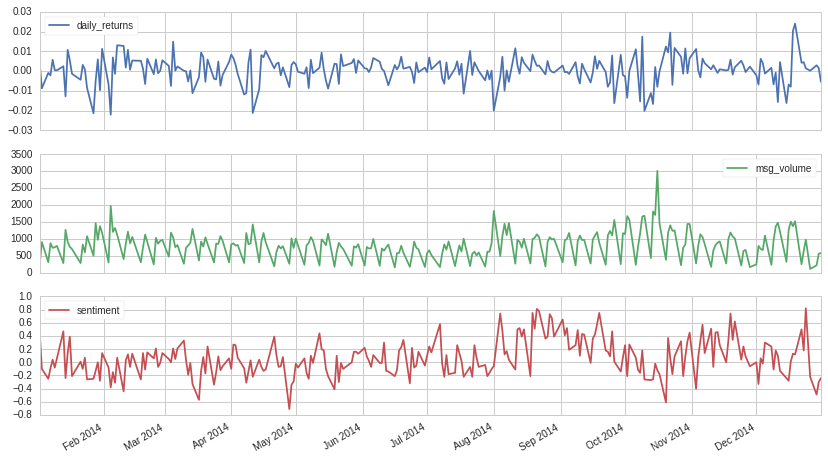
\includegraphics[width=0.5\textwidth]{research.png}
\caption{\label{fig:sol_iter}Gráfico con los datos incluidos en el pipeline del ambiente de investigación}
\end{figure}


\subsection{La clase Pipeline}
Esta clase permite:

\begin{itemize}
    \item Acceder a un conjunto de datos especificado de forma secuencial, para ser procesados por el algoritmo.
    \item Calcular métricas establecidas \textit{(factors)}, como por ejemplo retornos, medias móviles e indicadores de análisis.
\end{itemize}

Dentro del entorno de desarrollo, el primer paso es importar las librerías de clases. En este caso la clase Pipeline para la importación de datos a modo de flujo (no estático, como una tabla de pandas), la clase factors con los factores para calcular medias móviles, y medias móviles exponenciales ponderadas. De clase data se importa el conjunto de datos stocktwits.

Además, de la clase \textit{algorithm}, se importan objetos para conectar el objeto Pipeline y obtener sus datos

\lstset{columns=fullflexible, xleftmargin=1cm, basicstyle=\footnotesize, language=Python, breaklines=true, numbers=left} 
\begin{lstlisting}
from quantopian.algorithm import attach_pipeline, pipeline_output
from quantopian.pipeline import Pipeline
from quantopian.pipeline.factors import SimpleMovingAverage, EWMA
from quantopian.pipeline.data.psychsignal import stocktwits as psychsignal # Sentiment data
\end{lstlisting}

\subsection{Estructura del algoritmo}
De forma similar al usar zipline, los algoritmos en Quantopian deben implementar una serie de funciones estandarizadas para procesar los datos y realizar las ordenes, sin embargo no es necesario utilizar el paradigma de orientación a objetos

En este caso se hace uso de dos funciones estandarizadas, la función \textit{initialize}, que se ejecuta al iniciar el algoritmo, 

\begin{lstlisting}
def initialize(context):
    context.asset = symbol('SPY')
    sma = SimpleMovingAverage(inputs=[psychsignal.bull_minus_bear], window_length=5)
    ewma = EWMA.from_span(inputs=[psychsignal.bull_minus_bear], window_length=5, span=5)
    
    pipe_columns = {
        'sentiment':psychsignal.bull_minus_bear.latest,
        'msg_volume'  :psychsignal.total_scanned_messages.latest,
        'sma' :sma,
        'ewma' :ewma,
    }
    
    # Attaching our pipeline
    pipe = Pipeline(columns = pipe_columns)
    pipe = attach_pipeline(pipe, name='sentiment')
    schedule_function(rebalance, date_rules.every_day(), time_rules.market_open())
\end{lstlisting}

la funcion \textit{before\_trading\_start} se ejecuta en cada iteración del algoritmo, justo antes que se abra el mercado. En este caso se utiliza para obtener los datos del estado de animo del mercado, mas específicamente el campo \textit{sentiment} proveniente del pipeline definido antes, al cual se van a eliminar los valores nulos con el método dropna y filtrarlos para obtener solo los valores para el activo definido, es decir, para el S\&P500. 

\begin{lstlisting}
def before_trading_start(context, data):
    context.pipe = pipeline_output('sentiment').dropna().loc[context.asset]
\end{lstlisting}

Por ultimo, se define una función personalizada, la cual contiene las instrucciones para definir las posiciones en el activo y realizar las ordenes

La diseño de la estrategia de negociación es la siguiente:

\begin{itemize}
    \item \textit{Si} el ultimo valor del sentimiento del mercado es mayor a la media móvil calculada y no se tiene una posición en el activo, \textit{entonces} se toma una posición larga en este
    \item \textit{Si} el ultimo valor del sentimiento del mercado es menor a la media móvil calculada y se tiene una posición larga en el activo, \textit{entonces} liquide la posición en este
\end{itemize}

La implementación de esta estrategia en Quantopian es la siguiente:

\begin{lstlisting}
def rebalance(context, data):
    current_position = context.portfolio.positions[context.asset].amount
    buy = False
    sell = False
        
    # rebalance portfolio
    if context.pipe.sentiment > context.pipe.sma and current_position <= 0:
        order_target_percent(context.asset, 1)
        buy = True
        sell = False
    elif context.pipe.sentiment < context.pipe.sma and current_position >= 0:
        order_target(context.asset, 0)
        buy = False
        sell = True
        
    record(sentiment=context.pipe.sentiment, sma=context.pipe.sma, ewma=context.pipe.ewma)
    log.info("Sentiment: " + str(context.pipe.sentiment))
    log.info("sma: " + str(context.pipe.sma) + ", ewm: " + str(context.pipe.ewma))
\end{lstlisting}

Primero, se utiliza el objeto portfolio\footnote{https://www.quantopian.com/help\#api-portfolio}, el cual contiene varias propiedades relacionadas con el desempeño del portafolio de inversión, como los retornos, el dinero disponible para realizar operaciones (cash), el valor de este, y para este caso, la posición de los activos. Como puede verse, estas posiciones se guardan en una variable de tipo diccionario, al cual se accede con el identificador del activo seleccionado. Además se crean unas banderas booleanas para identificar las posiciones tomadas.

A continuación, se implementa la estrategia mediante una sentencia \textit{if} simple en la cual, utilizando el objeto pipe, se obtienen los valores del valor actual del sentimiento del mercado (pipe.sentiment) y el valor del promedio móvil definido al inicio (pipe.sma)

Para realizar las ordenes, en el caso de compra se utiliza la función \textit{order\_target\_percent}, con la cual se establece una posición en el activo en términos porcentuales del dinero disponible en el portafolio. La cantidad del activo se define con valores entre 0 y 1.

Por ultimo, para verificar la ejecución de la estrategia, se realiza un registro de los valores del estado de animo del mercado, la media móvil calculada, y el valor de la media móvil exponencial calculada, para mostrarse en el panel gráfico con la función \textit{record}. Con la función \textit{log}, se crea un registro para guardar los valores anteriores en la consola.

\section{Conclusiones}
Esta estrategia podría entenderse como una versión simplificada de un análisis de sentimiento, en la medida que las tendencias de búsqueda de un termino están relacionadas con un sentimiento positivo o negativo sobre la ocurrencia de algún evento o hecho. De esta forma, dichas tendencias pueden estar relacionadas con los comportamientos de activos financieros. Esta relación puede verse con el ejemplo propuesto de las tendencias de QE y el indice NYSE Composite.

También hay que tener en cuenta otros posibles indicadores a aplicar sobre los datos de tendencias, que puedan mejorar el desempeño de la estrategia de inversión.

Otro posible escenario podría ser utilizar dos tendencias de términos que sean uno opuesto al otro, y realizar una estrategia de tipo \textit{Pairs Trading}.
\end{document}


